\documentclass[12pt]{beamer}
\usepackage[T1]{fontenc}
\usepackage[utf8]{inputenc}
\usetheme[]{Honefoss}
\usepackage{hyperref}
\hypersetup{
    colorlinks=true,
    linkcolor=blue,
    filecolor=magenta,      
    urlcolor=cyan,
}

\urlstyle{same}

\title{Where}
\subtitle{A geodetic software}
\author{Ingrid Fausk, Michael D\"ahnn, Ann-Silje Kirkvik}
\date{May 4, 2020}

\begin{document}
\frame{\titlepage}

\begin{frame}{Introduction}
\begin{itemize}
\item
  \textit{Where} is a Python software package used for analyzing VLBI, SLR and GNSS data
\item
  \textit{Where} is currently being developed at the Norwegian Mapping Authority (NMA)
\item
  \textit{Where} is an open source project, available on github \url{https://github.com/kartverket/where}
\end{itemize}
\end{frame}


\begin{frame}{International collaboration}
\begin{itemize}
\item 
  NMA has a cooperation agreement with IGN of Spain and the Yebes observatory
\item 
  IGN provides the receivers and technical assistance for the VLBI antennas in Ny-{\AA}lesund
\item 
  NMA provides the \textit{Where} analysis software and support for the analysis group at IGN
\end{itemize}
\end{frame}


\begin{frame}{Analysis Center}
\begin{itemize}
\item
  NMA is associated analysis center within the IVS and ILRS. Both the NMA and IGN,
  are in a test phase of deliveries of VLBI analysis results to the IVS
  with the Where software. Some of our activities in VLBI is documented
  in~\cite{kirkvik2017b} and~\cite{kirkvik2018}
\item
  Our goal is to be able to contribute to the ILRS after some improvements of the
  software, and in the future receive full status as operational analysis center
  for both VLBI and SLR
\end{itemize}
\end{frame}


\begin{frame}{Technology}

The \textbf{Where} software is mainly being written in \emph{Python}

\begin{itemize}
\item
  Solid, flexible and fast libraries like \texttt{numpy},
  \texttt{matplotlib} and \texttt{scipy} are available
\item
  We use a \textbf{HDF5}-based format for storing data
\item
  Python has effective interfaces to \emph{C} and \emph{Fortran}
  code, and we can use the \textbf{Sofa} and \textbf{IERS} software
  libraries directly
\end{itemize}
\end{frame}

\begin{frame}{The Where Pipeline}

The pipelines for the different techniques are shown in the figure below. 

\begin{center}
  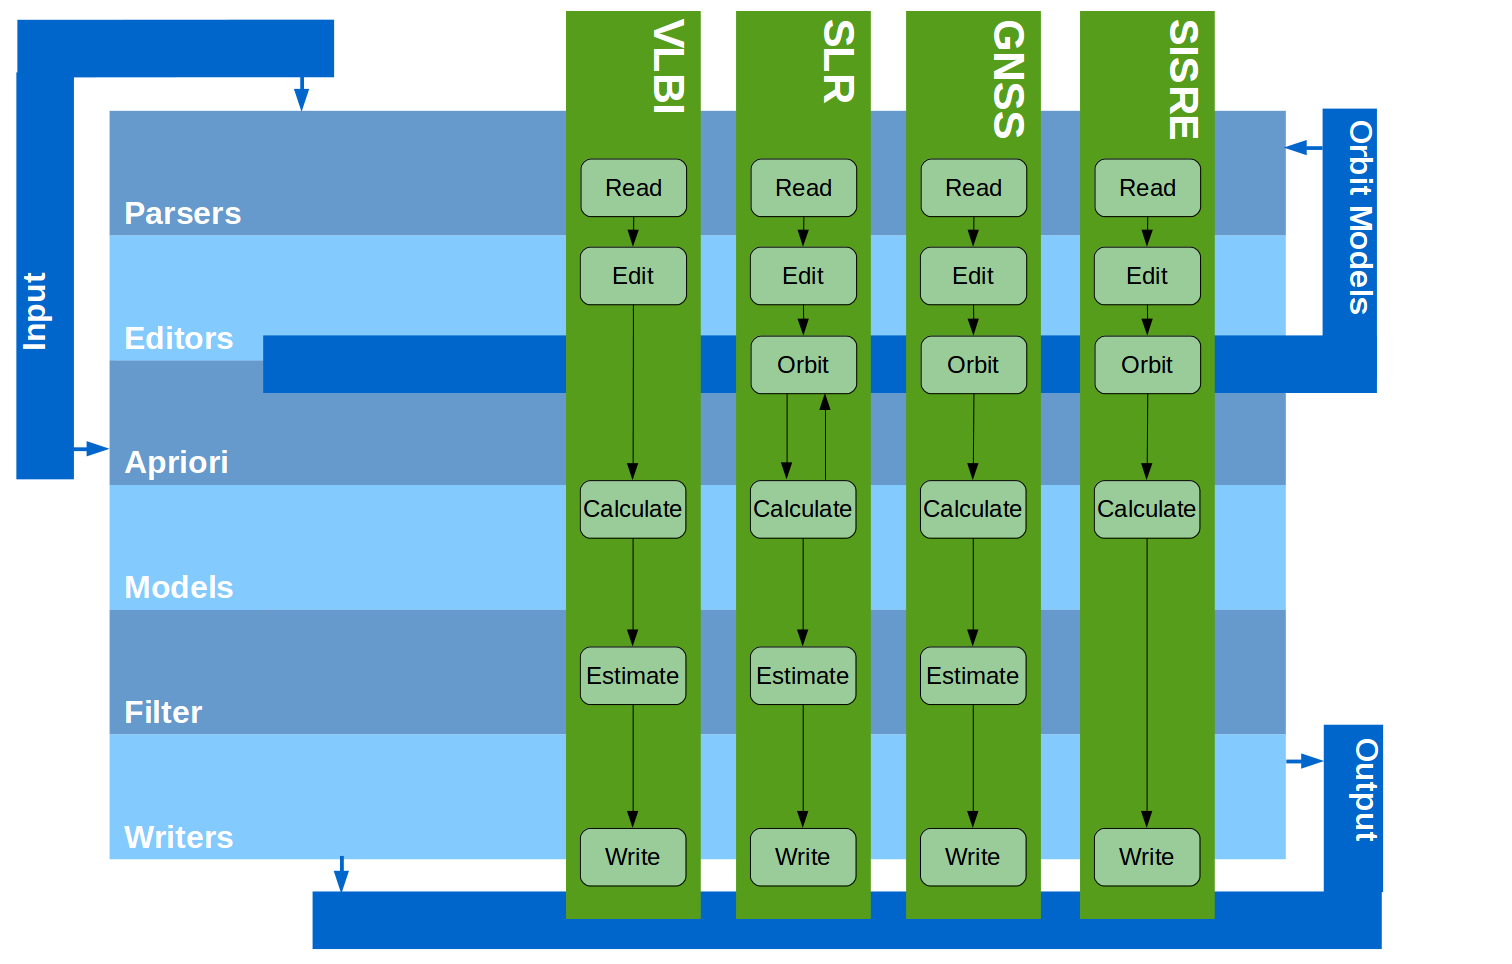
\includegraphics[height=0.7\textheight]{./figure/pipelines.png}
\end{center}

\end{frame}

\begin{frame}{Models}
\begin{itemize}
\item
  The implementation of the individual models follow the 2010 IERS Conventions, see \url{www.iers.org/IERS/EN/Publications/TechnicalNotes/tn36.html}
\item
  When possible we have used software libraries made available at the IERS ftp page \url{ftp://maia.usno.navy.mil/conventions/2010} 
\item 
  The estimation of EOP parameters and station positions is done using a Kalman filter~\cite{mysen2017}. We use continuous piecewise linear functions for the estimation
\end{itemize}
\end{frame}

\begin{frame}{Orbit determination}
\begin{itemize}
\item
  Force models, variational equations and orbit estimation is computed following Montenbruck and Gill~\cite{montenbruck2012}
\item 
  Cowell orbit integrator following Oesterwinter and Cohen~\cite{oesterwinter1972} 
\item
  The observation equation for SLR is following Beutler~\cite{beutler2005}
\item
  All models are implemented, but...
\begin{itemize}
\item 
  Orbit residuals are a few centimeters too large, so we are currently debugging the orbit models
\item
  The orbit determination is a bit slow
\end{itemize}
\end{itemize}
\end{frame}

\begin{frame}{Useful Features}
\begin{itemize}
\item
  Logging of events that occur while software runs. 
\item 
  Configuration files defines the details on how the analysis is done. Examples include what data is used, how to clean the data before analysis and which parameters to estimate.
\item 
  Dataset with time objects, position and velocity objects, including conversion routines. 
\end{itemize}
\end{frame}
 

\begin{frame}{There}

\textit{Where} is a command line tool, but the results can be inspected using the graphical tool called \textit{There}. A screenshot is shown below.

\begin{center}
  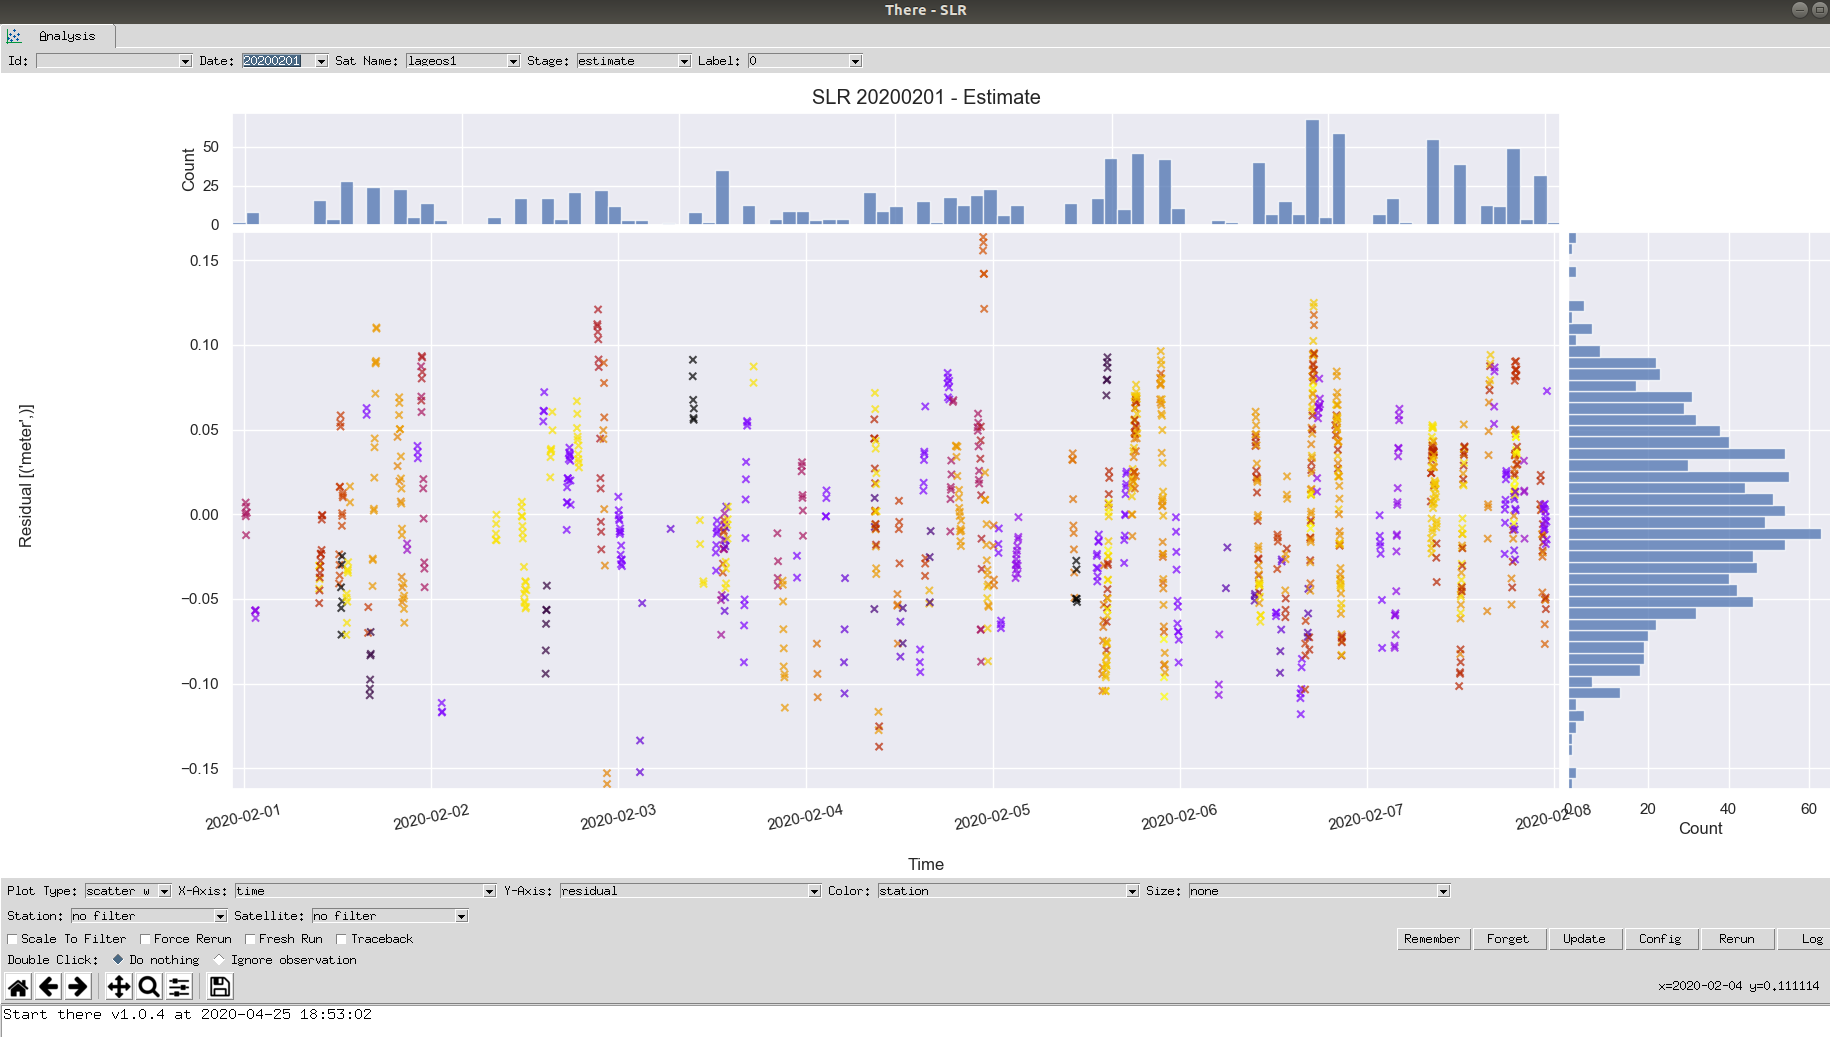
\includegraphics[height=0.6\textheight]{./figure/there.png}
\end{center}
\end{frame}


\begin{frame}{Using Where}
\begin{itemize}
\item 
  MIT Open Source License: Permissive, use Where as you want
\item
  But please acknowledge us if you use Where
\item 
  Get in touch if you are interested in Where
\end{itemize}
\end{frame}


\begin{frame}{References}
\tiny
\bibliographystyle{../../where}
\bibliography{../../where}

\end{frame}
\end{document}
